% !TEX root = ../my_thesis.tex

\section{Training des Convolutional Neural Networks}
Künstliche neuronale Netze bzw. CNNs werden grundsätzlich zuerst aufgabenspezifisch modelliert und anschließend mit entsprechenden Daten trainiert.  In der vorliegenden Arbeit wird als Netzwerk das in Abschnitt \ref{sec:posenet} beschriebene PoseNet Model verwendet. Die Arbeit folgt den Ansatz von \citet{acharyaBIMPoseNetIndoorCamera2019} mit Gradienten- bzw. Kantenbilder der synthetischen Daten das Netzwerk zu trainieren, um anschließend mit Gradientenbilder der realen Daten das Netzwerk zu evaluieren. 

Im weiteren Verlauf dieses Kapitel werden die verwendeten Datensätze gelistet, die Erhebung bzw. Generierung der realen bzw. synthetischen Daten beschrieben, die Verarbeitung der Daten dargestellt und die Trainingsparameter angegeben. 


\subsection{Datensätze}
\label{subsec:datasets}
In dieser Arbeit werden aus zwei unterschiedlichen Gebäuden Daten erhoben bzw. synthetische Daten aus den Gebäudesimulationen generiert. 
Der erste Datensatz a) beinhaltet Daten der nördliche Hälfte des 6. Stockwerkes der IC-Gebäude Ruhr-Universität Bochum. Der zweite Datensatz b) beinhaltet Daten der Seminargebäude Hochschule Bochum.
TODO

trajectory images


\begin{table}[H]
	\centering
	\caption{Übersicht der Datensätze.}
	\begin{tabularx}{1.0\textwidth}{X X X >{\centering\arraybackslash}p{1.7cm} }
		\textbf{Bezeichnung} & \textbf{Streckenlänge} & \textbf{Volumen} & \textbf{Gebäude}\\
		\hline
		IC-loop & 115$m$ & $50m \times 11m \times 3.5m$ & a) \\
		\hline
		HS-stairs & 115$m$ & $30m \times 30m \times 30m$ & a)\\
		\hline
		HS-floor & 115$m$ & $30m \times 30m \times 30m$ & a)\\
	\end{tabularx}
	\label{tab:dataset_metrics}
\end{table}

\begin{table}[H]
	\centering
	\caption{Übersicht der Datensätze.}
	\begin{tabularx}{1.0\textwidth}{p{3.5cm} p{1.8cm} X  >{\centering\arraybackslash}p{1.7cm} }
		\textbf{Bezeichnung} & \textbf{Typ} & \textbf{Anzahl Daten} (davon verwendet) & \textbf{Gebäude}\\
		\hline
		IC-loop & real & 3842 (3000) & a) \\
		\hline
		IC-loop-syn & synth. & 11435 (11000) & a)\\
		\hline
		HS-stairs-up & real & 1068 (1000) & b)\\
		\hline
		HS-stairs-up-syn & synth & 3160 (3000) & b)\\
		\hline
		HS-stairs-down & real & 1161 (1000) & b)\\
		\hline
		HS-stairs-down-syn & synth &  3245 (3000) & b)\\
		HS-loop & real & 1161 (1000) & b)\\
		\hline
		HS-loop-syn & synth &  3245 (3000) & b)\\
	\end{tabularx}
	\label{tab:datasets}
\end{table}

\cleardoublepage
\subsection{Erhebung der realen Daten}
\label{subsec:record_real_data}
In der Literatur wurden die realen Daten einer Zone grundsätzlich entlang einer Strecke aufgenommen \cite{kendallPoseNetConvolutionalNetwork2015, clarkVidLocDeepSpatioTemporal2017, acharyaBIMPoseNetIndoorCamera2019}. Daher werden für die Aufgabenstellung interessante Aufnahmestrecken in den Gebäudesimulationen festgelegt und anschließend die Aufnahmen so durchgeführt, dass diverse Projekte damit Forschung betreiben können. 

In der Literatur wurden SfM-Methoden eingesetzt, um die Ground-Truth-Daten der realen Aufnahmen zu bestimmen \cite{kendallPoseNetConvolutionalNetwork2015, clarkVidLocDeepSpatioTemporal2017, acharyaBIMPoseNetIndoorCamera2019}. 
In der vorliegenden Arbeit wird für die Bestimmung der Ground-Truth-Daten sowie die Aufnahme der Bilder zeitgleich zwei unterschiedliche Kameras der Intel Realsense Reihe verwendet. Eine Intel Realsense T265\footnote{\url{https://www.intelrealsense.com/tracking-camera-t265/} (abgerufen am: 18.07.2019)} wird eingesetzt, die die Odometrie (Ground-Truth-Daten) mit einer Abweichung von 1\%  über die SfM von zwei Fischaugenkameras und Inertial Measurement Units (\textit{IMU}) ermittelt. Zudem wird eine Intel Realsense D435\footnote{ \url{https://www.intelrealsense.com/depth-camera-d435/} (abgerufen am: 18.07.2019)} eingesetzt, die eine 3D Punktwolke, ein Tiefenbild sowie ein RGB-Bild einer Szene liefert. Die T265 wird über die D435 Kamera montiert (siehe Abbildung \ref{fig:t265_d435}). 

\begin{figure}[H]
	\centering
	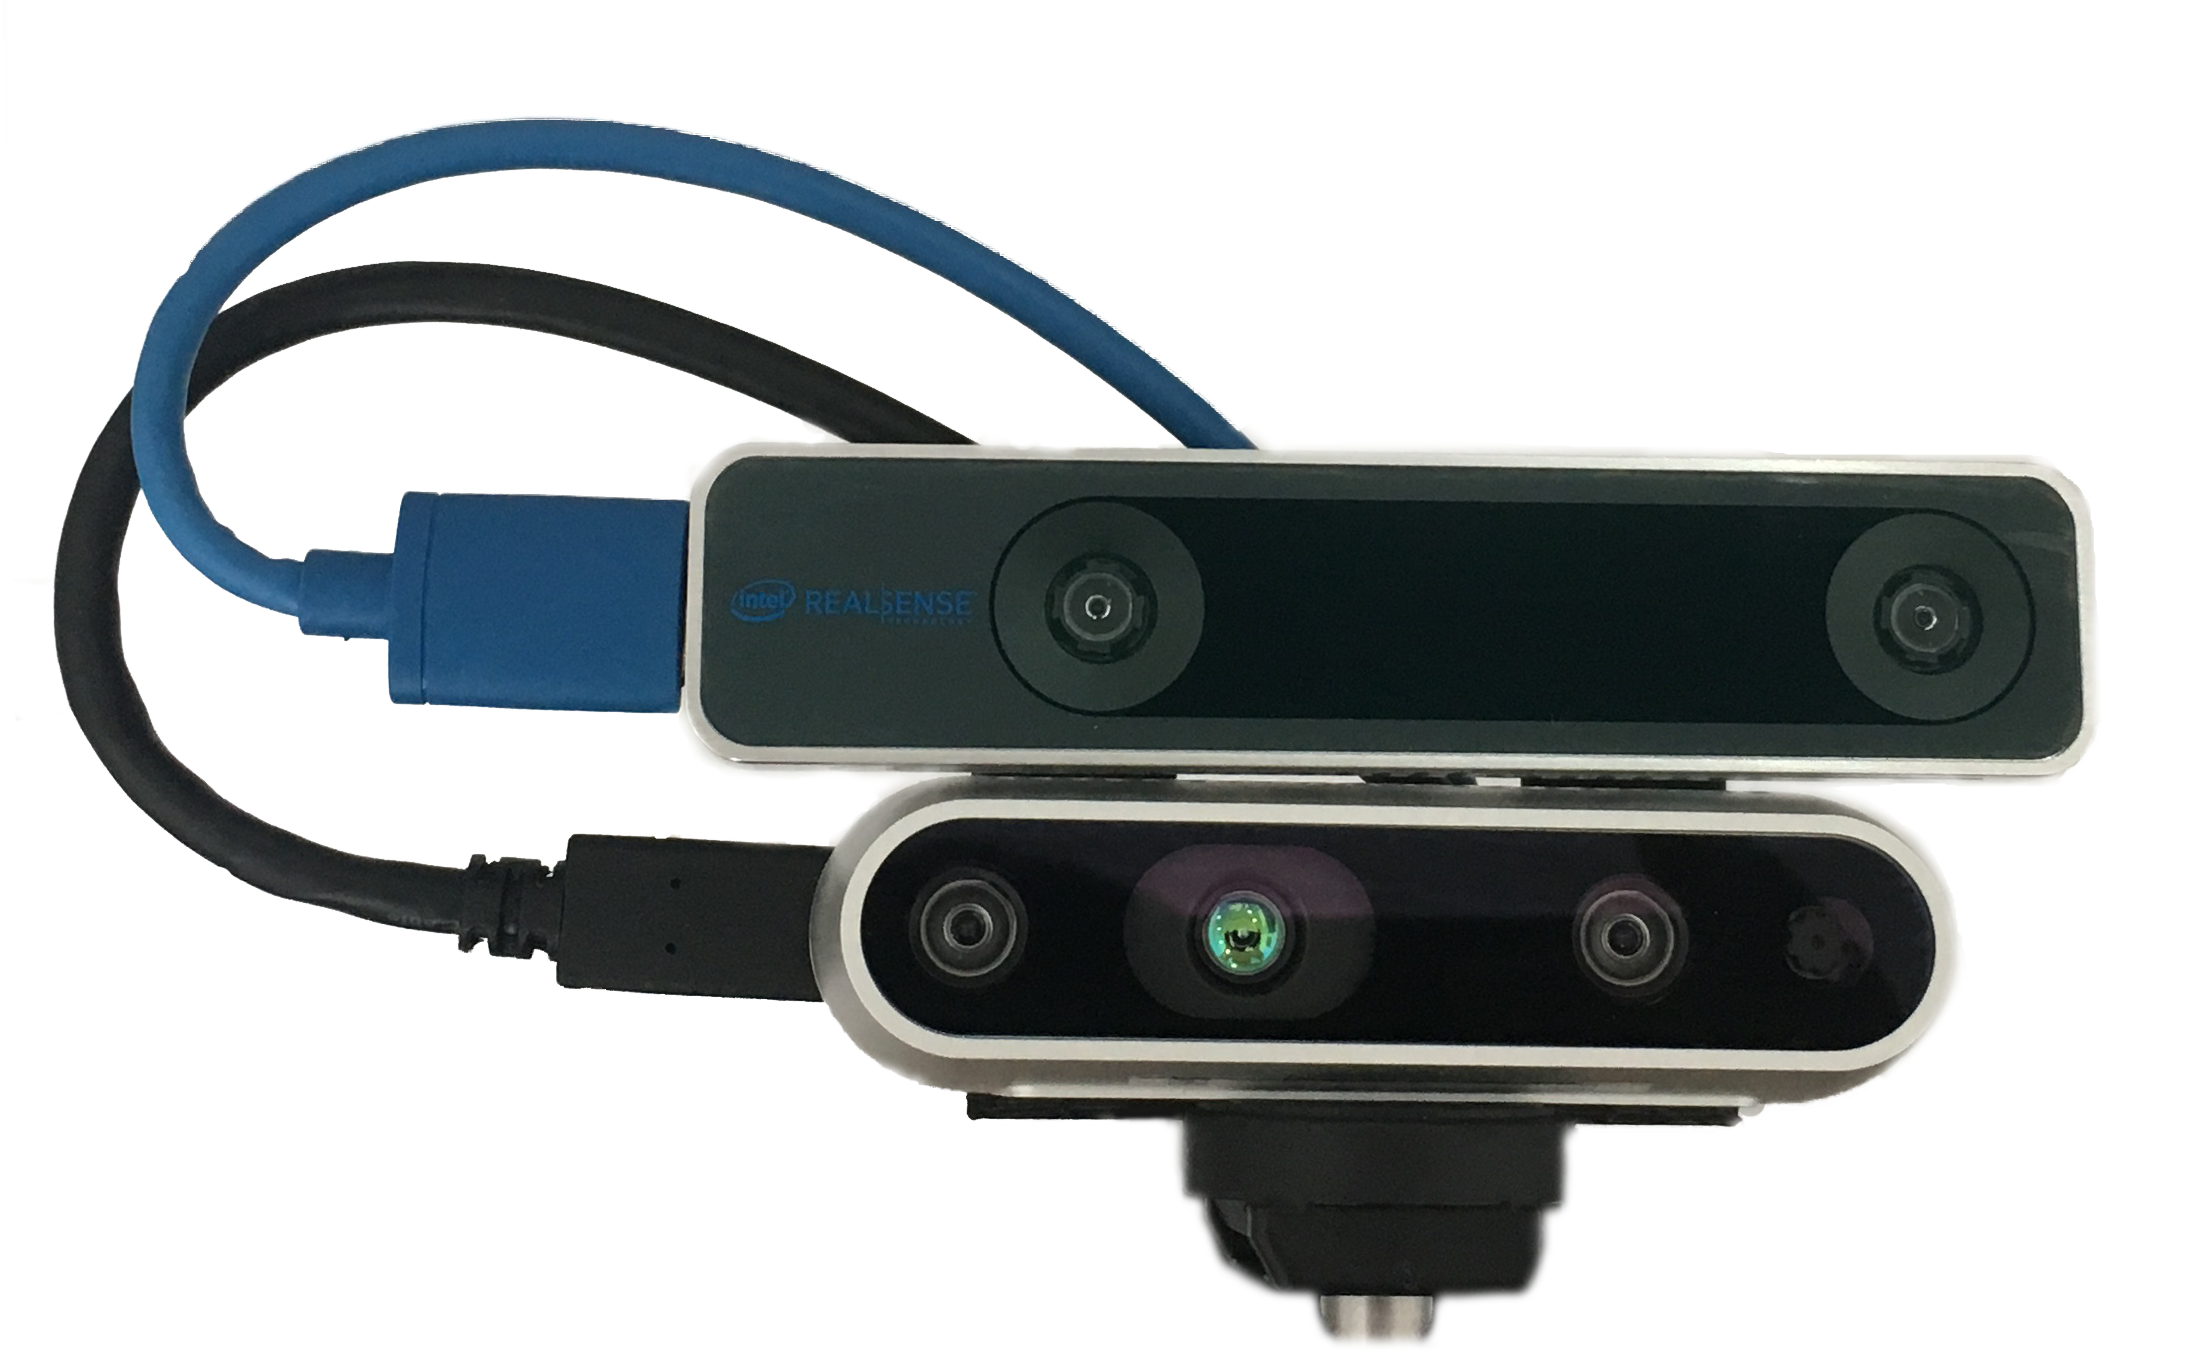
\includegraphics[width=0.5\textwidth]{images/real_dataset/t265_d435_2.png}
	\caption{Hardware für die Aufnahme der realen Daten. Die Intel Realsense T265 ist oberhalb der Intel Realsense D435 montiert. Das Konstrukt kann auf einer universalen Stativschraube befestigt werden.  }
	\label{fig:t265_d435}
\end{figure}

Über das Robot Operating System\footnote{\url{https://www.ros.org/about-ros/} (abgerufen am: 18.07.2019)} (\textit{ROS}) Framework werden die Kameras zeitgleich angesprochen und der Datenfluss der Kameras synchronisiert. Somit beinhaltet jeder Datensatz ein Bild je Fischaugenkamera, ein Tiefenbild, ein RGB-Bild, eine 3D Punktwolke und die dazugehörige Odometrie pro Frame. Für die vorliegende Arbeit sind nur die Odometrie-Daten der T265 sowie die RGB-Bilder der D435 relevant. Die Abbildung \ref{fig:dataset} visualisiert ein Datensatzexemplar für ein Frame.


\begin{figure}[H]
	\centering
	\begin{subfigure}[t]{0.3\linewidth}
		\centering
		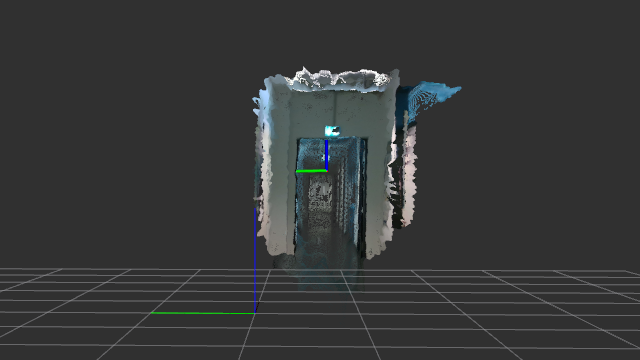
\includegraphics[width=\linewidth]{images/real_dataset/pointcloud3.png}
		\caption{Odometrie  (T265) + \\ 3D Punktwolke (D435)}
		\label{subfig:odom1}
	\end{subfigure}
	\hfill
	\begin{subfigure}[t]{0.3\linewidth}
		\centering
		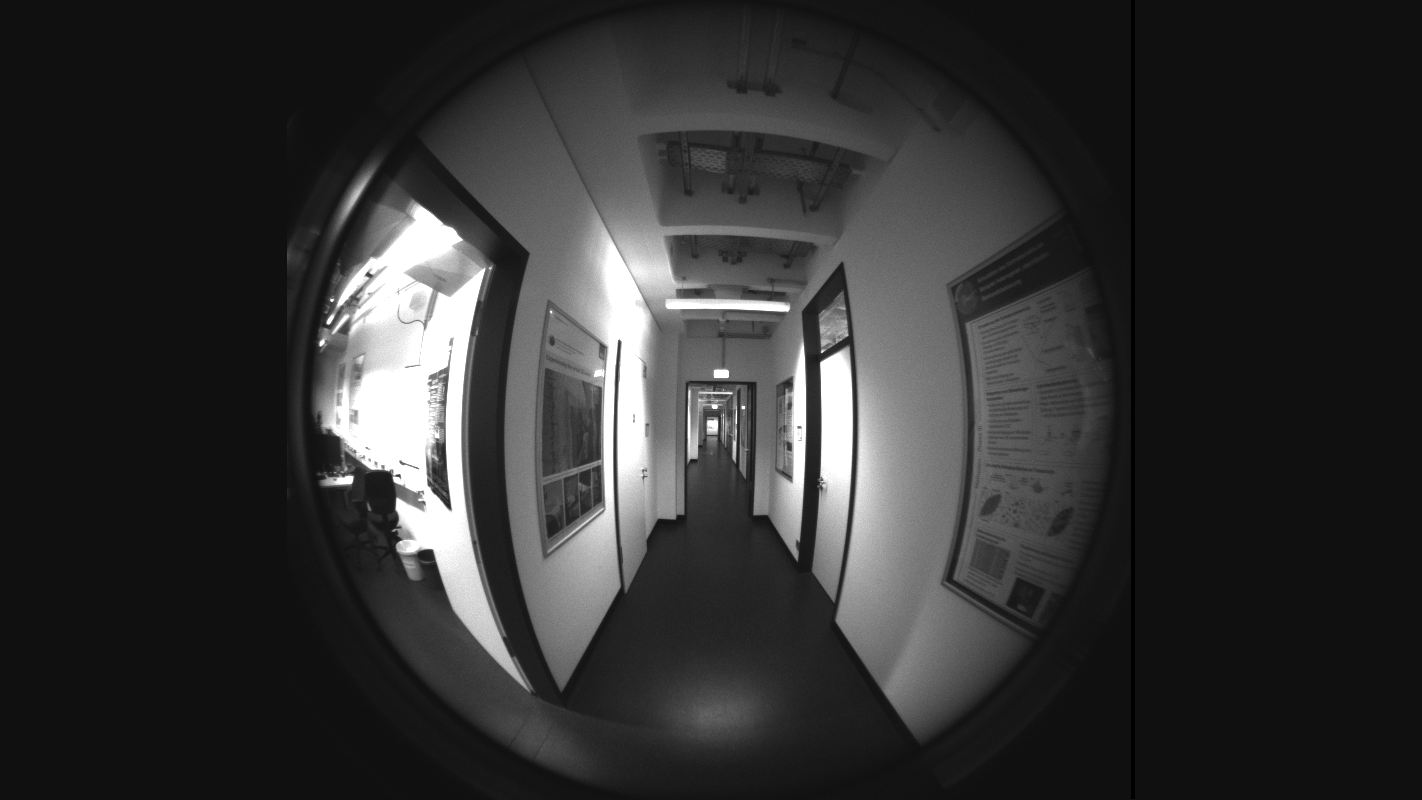
\includegraphics[width=\linewidth]{images/real_dataset/f1_frame000005.png}
		\caption{Fischaugenkamera 1 \\ (T265)}
		\label{subfig:fisheye1}
	\end{subfigure}
	\hfill
	\begin{subfigure}[t]{0.3\linewidth}
		\centering
		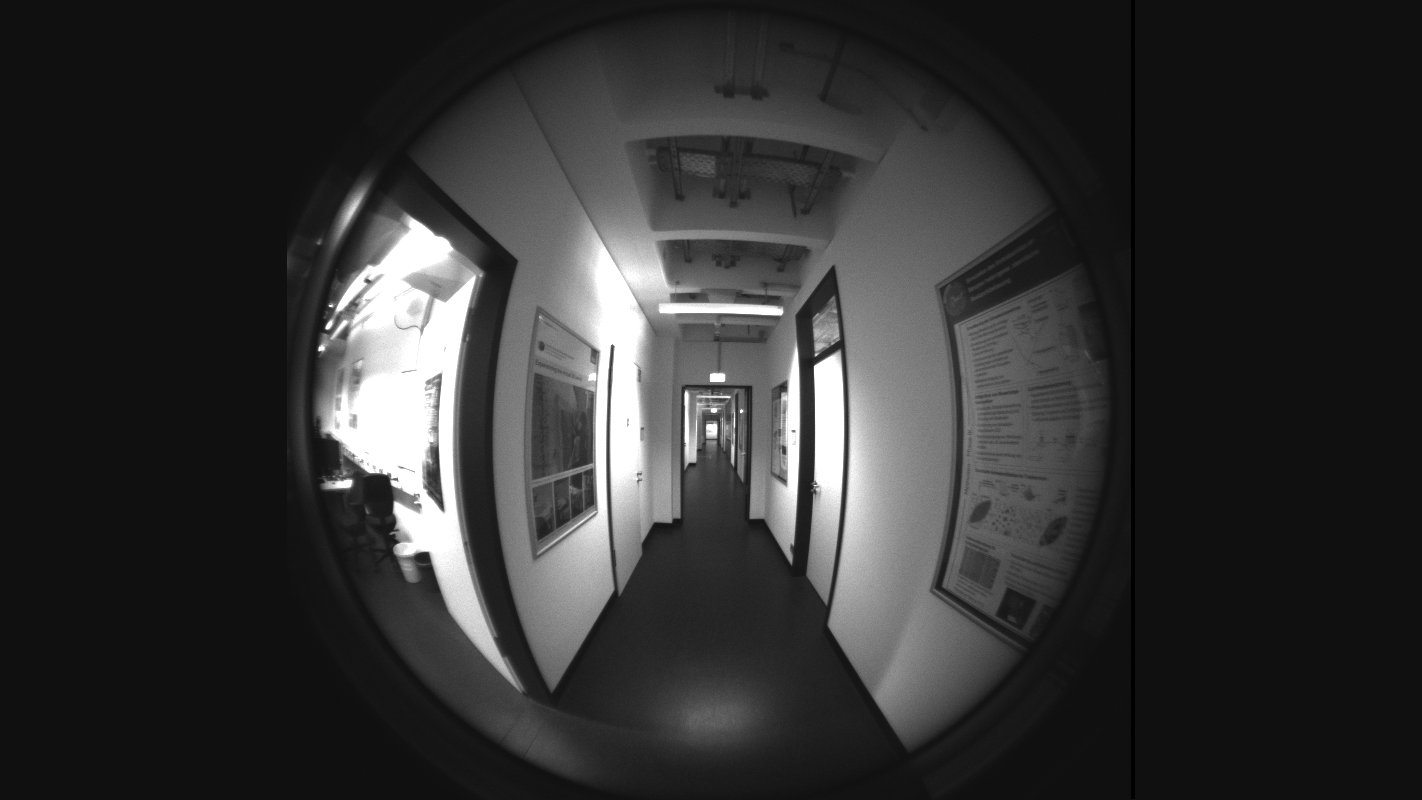
\includegraphics[width=\linewidth]{images/real_dataset/f2_frame000005.png}
		\caption{Fischaugenkamera 2 \\ (T265)}
		\label{subfig:fisheye2}
	\end{subfigure}
	\hfill \medskip
	\begin{subfigure}[t]{0.3\linewidth}
		\centering
		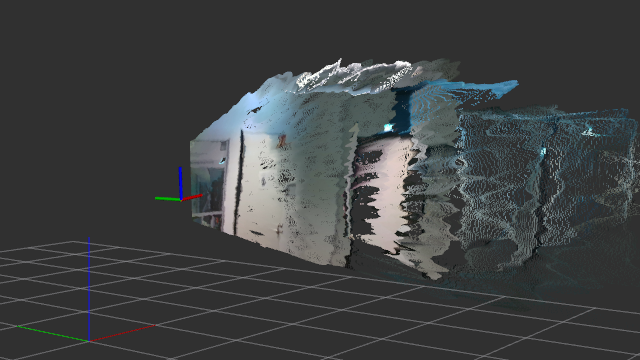
\includegraphics[width=\linewidth]{images/real_dataset/pointcloud1.png}
		\caption{Odometrie  (T265) + \\ 3D Punktwolke (D435)}
		\label{subfig:odom2}
	\end{subfigure}
	\hfill
	\begin{subfigure}[t]{0.3\linewidth}
		\centering
		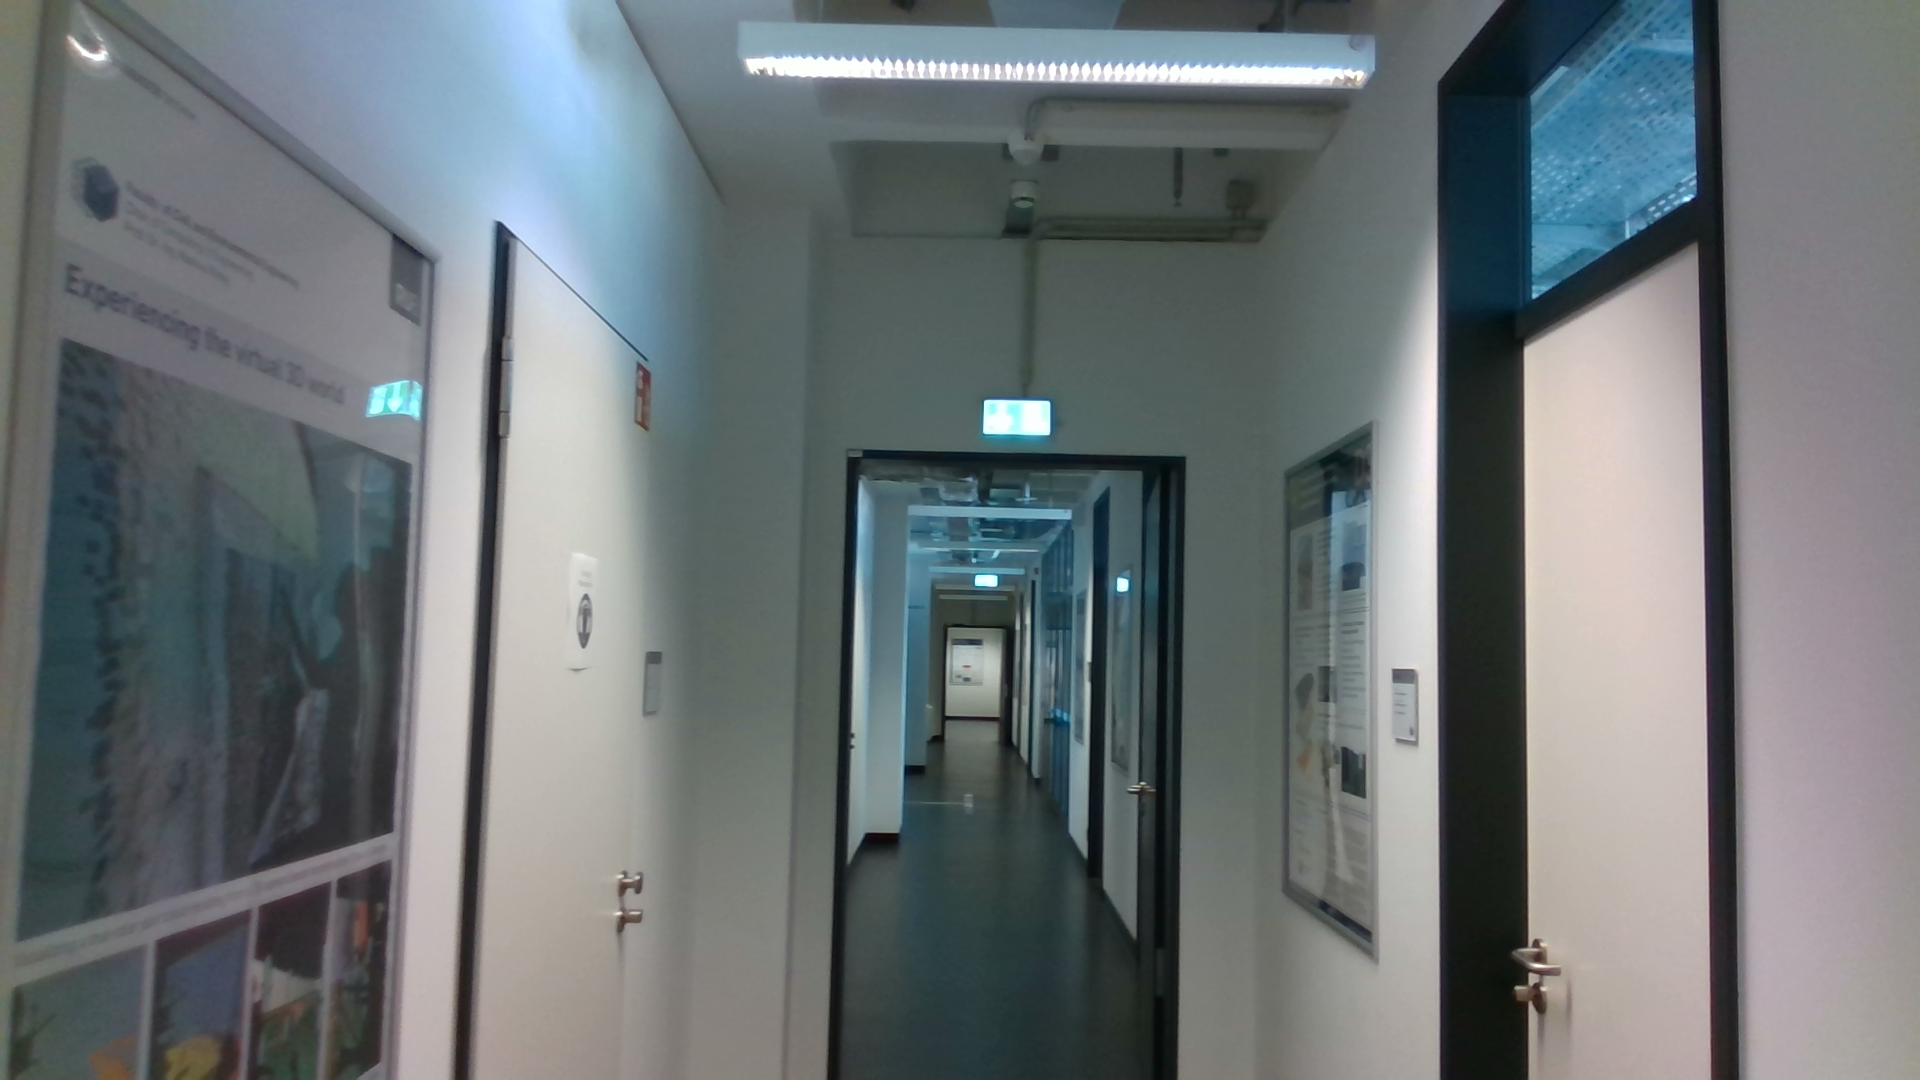
\includegraphics[width=\linewidth]{images/real_dataset/dc_frame000005.png}
		\caption{RGB-Bild \\ (D435) \hspace*{2cm}}
		\label{subfig:rgb-image}
	\end{subfigure}
	\hfill
	\begin{subfigure}[t]{0.3\linewidth}
		\centering
		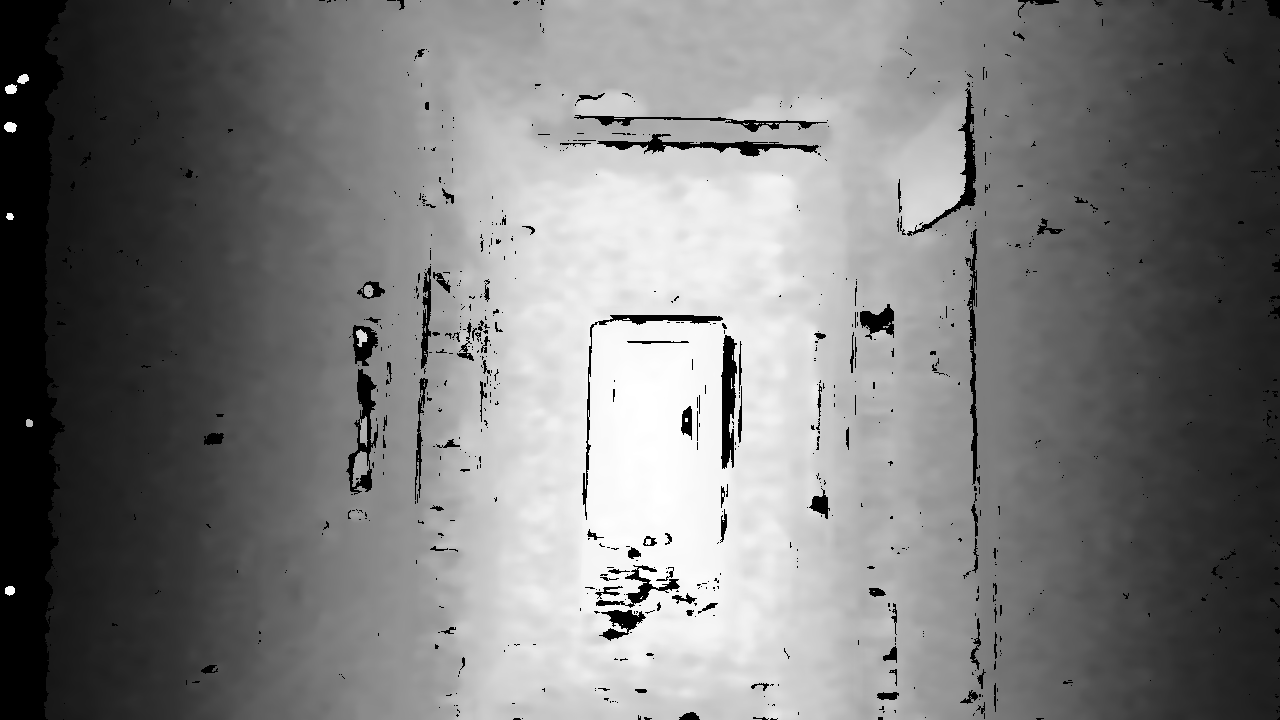
\includegraphics[width=\linewidth]{images/real_dataset/dt_frame000005.png}
		\caption{Tiefenbild \\ (D435) \hspace*{2cm}}
		\label{subfig:depth-image}
	\end{subfigure}
	\caption{Datensatz pro Frame. \ref{subfig:odom1}  und \ref{subfig:odom2} visualisieren in unterschiedlichen Prespektiven die von der T265 ermittelte Odometrie und die von der D435 erhaltenen 3D Punktwolke. \ref{subfig:fisheye1} und \ref{subfig:fisheye2} sind die von der T265 aufgenommenen Fischaugenbilder. \ref{subfig:rgb-image} ist das RGB-Bil der D435 und \ref{subfig:depth-image} das dazugehörige Tiefenbild. }
	\label{fig:dataset}
\end{figure}


\subsection{Generierung der synthetischen Daten}
\label{subsec:generate_synth_images}

Die Gebäude werden in Blender\footnote{\url{https://www.blender.org/about/} (aufgerufen am: 20.07.2019)} Version 2.79b simuliert. Die intrinsischen Daten der D435 RGB-Kamera werden auf die virtuellen Kameras übertragen.

Die Strecke der echten Aufnahmen werden in den Simulationen schwankungslos auf einer konstanten Höhe von 1.70$m$ imitiert. Es wird entlang der Strecke in 0.05$m$ Intervallen und mit einer $\pm$10° Neigung in je y- und z-Achse Bilder mit korrespondierenden Ground-Truth-Daten aufgenommen. Die Abbildung \ref{fig:dataset_variation} illustriert die Variationen der Pose pro Stützpunkt auf einer Strecke.


\begin{figure}[H]
	\centering
	\begin{subfigure}[t]{0.18\linewidth}
		\centering
		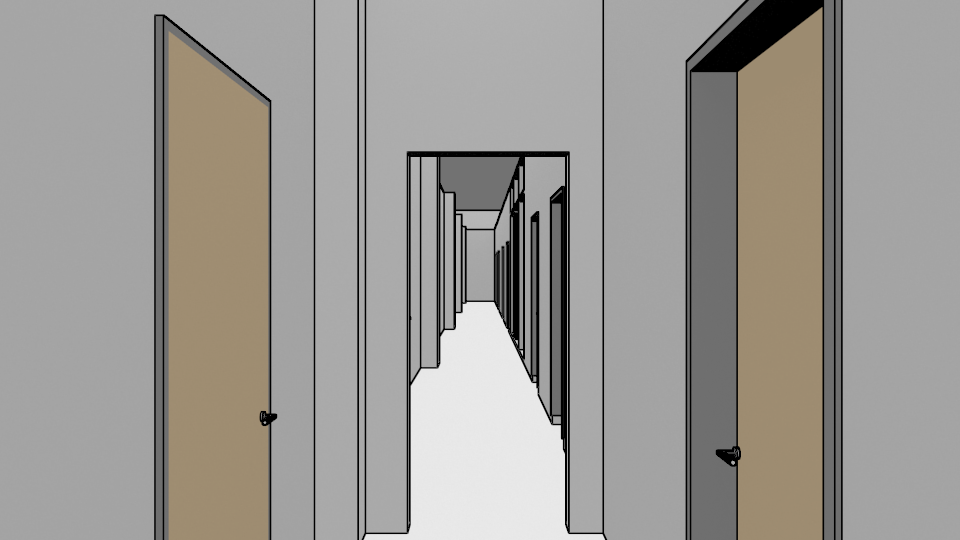
\includegraphics[width=\linewidth]{images/syn_dataset/00023.png}
		\caption{Orginal Pose \vspace{\fill}}
		\label{subfig:iz0_y0}
	\end{subfigure}
	\hfill 
	\begin{subfigure}[t]{0.18\linewidth}
		\centering
		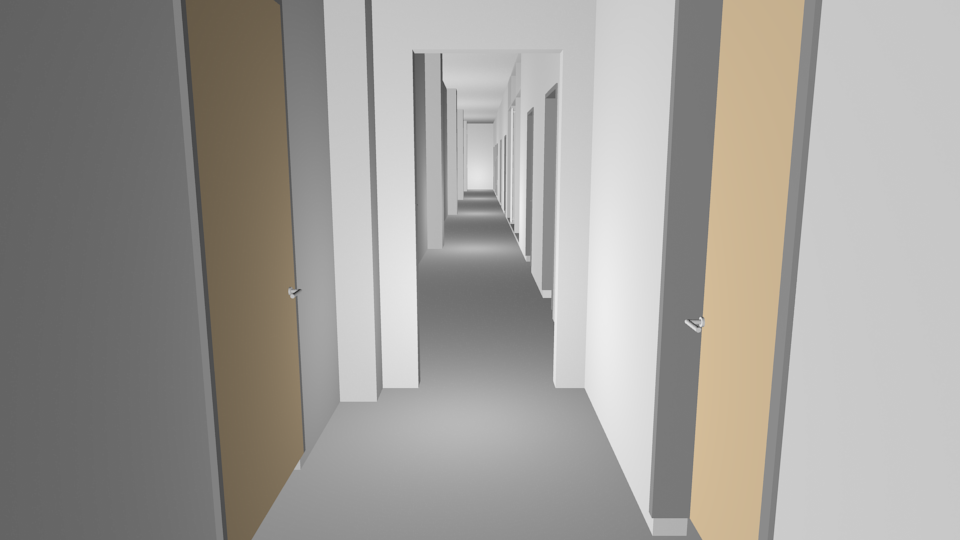
\includegraphics[width=\linewidth]{images/syn_dataset/00021.png}
		\caption{-10° um die y-Achse}
		\label{subfig:iz0_y-10}
	\end{subfigure}
	\hfill
	\begin{subfigure}[t]{0.18\linewidth}
		\centering
		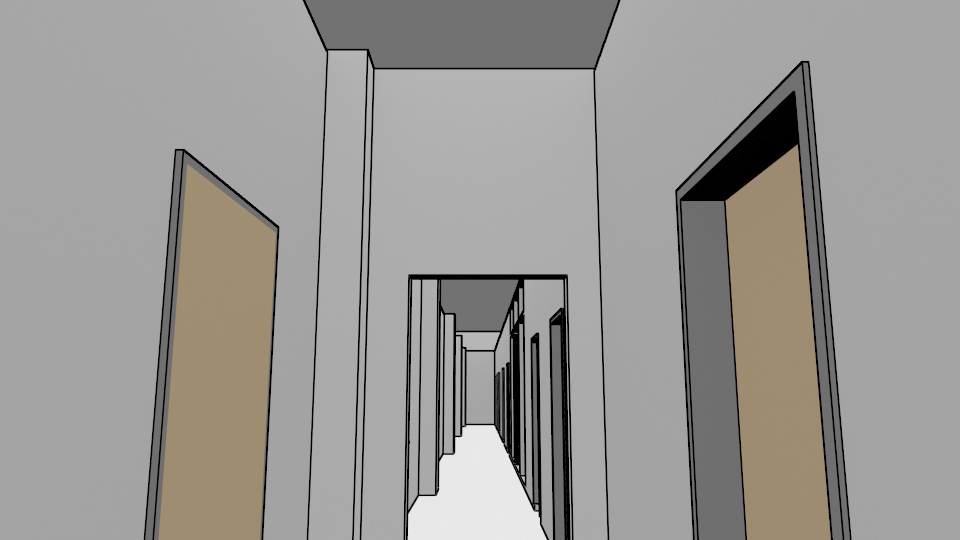
\includegraphics[width=\linewidth]{images/syn_dataset/00020.png}
		\caption{+10° um die y-Achse}
		\label{subfig:iz0_y+10}
	\end{subfigure}
	\hfill
	\begin{subfigure}[t]{0.18\linewidth}
		\centering
		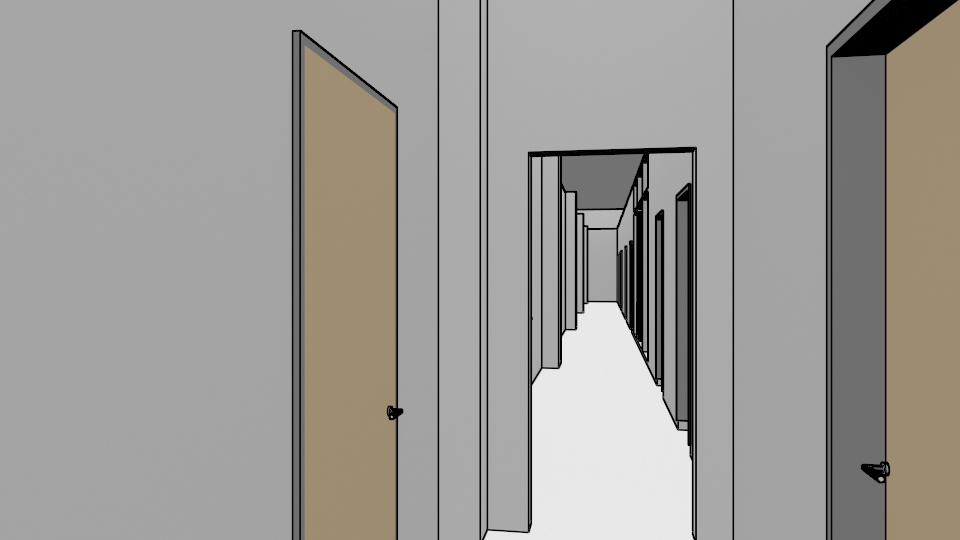
\includegraphics[width=\linewidth]{images/syn_dataset/00024.png}
		\caption{-10° um die z-Achse}
		\label{subfig:iz-10_y0}
	\end{subfigure}
	\hfill
	\begin{subfigure}[t]{0.18\linewidth}
		\centering
		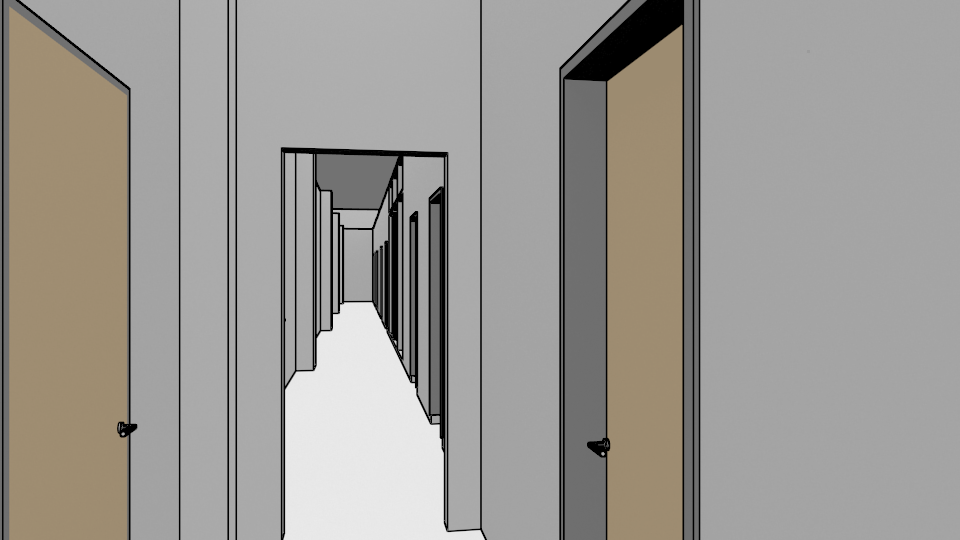
\includegraphics[width=\linewidth]{images/syn_dataset/00022.png}
		\caption{+10° um die z-Achse}
		\label{subfig:iz+10_y0}
	\end{subfigure}
	\caption{Variation der Pose pro Stützpunkt auf einer Strecke.}
	\label{fig:dataset_variation}
\end{figure}

Insgesamt werden drei synthetische Datensätze je Strecke erzeugt, die sich in der Beschaffenheit von \begin{enumerate*}[label=\alph*)]
	\item karikaturistische Darstellung zu
	\item synthetischen Kantenbilder hin über zu
	\item fotorealistische Darstellung
\end{enumerate*} unterscheiden (siehe Abbildung \ref{fig:dataset_preprocess}). Bei der Generierung der a) karikaturistischen und c) fotorealistischen Datensätzen wird die Beleuchtung aus einem Netz von Punktlichtquellen nachgestellt. Die a) karikaturistische und c) fotorealistische Datensätze unterscheiden sich ausschließlich in den Render-Engines.
Für die Erzeugung der b) synthetischen Kantenbilder wird eine konstante Beleuchtung verschaffen und die Kanten über Blender markant sichtbar konfiguriert. Der a) karikaturistische Datensatz sowie die b) Kantenbilder werden über die Render-Engine \textit{Blender Render} und der c) fotorealistischer Datensatz über die \textit{Cycles-Engine} generiert.



\subsection{Verarbeitung der Daten}
In der vorliegenden Arbeit wird PoseNet mit Gradientenbilder trainiert und evaluiert. Nach der Erhebung der realen Bilder (siehe Abschnitt \ref{subsec:record_real_data}) und Generierung der synthetischen Bilder (siehe Abschnitt \ref{subsec:generate_synth_images}) werden diese in ihre Gradientenbilder verarbeitet. 
(Vor der Verarbeitung in Gradientenbilder werden die Bilder auf eine Größe von $x \times y$ verkleinert.)

%Bei der Erzeugung von Gradientenbilder gehen einerseits wichtige Informationen im Hinblick auf das Ursprungsbild verloren, andererseits bleiben wichtige Informationen wie z.B. die geometrische Struktur erhalten.

Es wird zusätzlich ein Schwellenwertverfahren mit einer Schwelle von 64 angewendet, um unerwünschter Artefakte zu unterdrücken, sodass alle Pixeln im Wertebereich $[64, 255]$ liegen. Die Abbildung \ref{fig:dataset_preprocess} visualisiert von jedem Datensatztyp ein Beispiel und die dazugehörigen Gradientenbilder.

\vspace{\fill}
\begin{figure}[htp]
	\centering
	\begin{subfigure}[t]{0.24\linewidth}
		\centering
		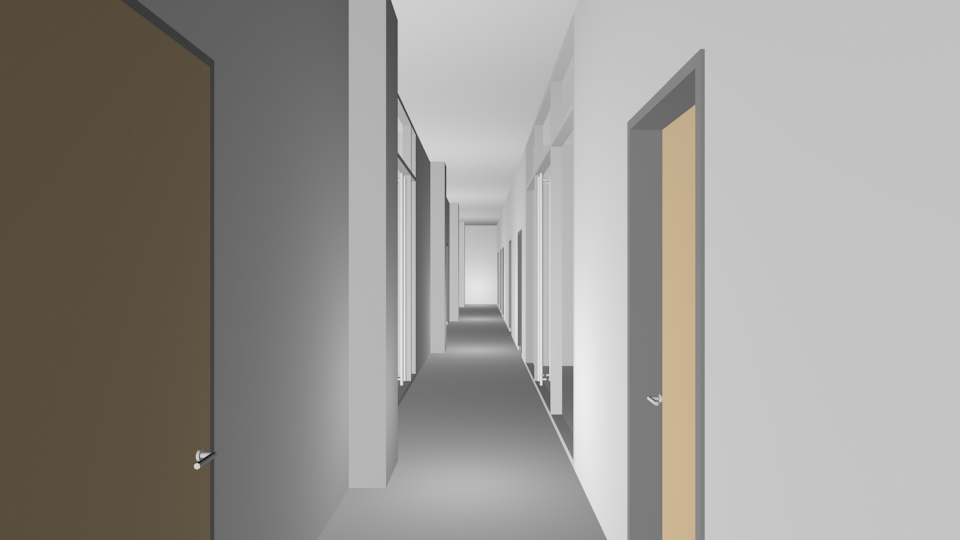
\includegraphics[width=\linewidth]{images/syn_dataset/b00708.png}
		\caption{karikaturistische Simulation}
		\label{subfig:cartoonish}
	\end{subfigure}
	\hfill
	\begin{subfigure}[t]{0.24\linewidth}
		\centering
		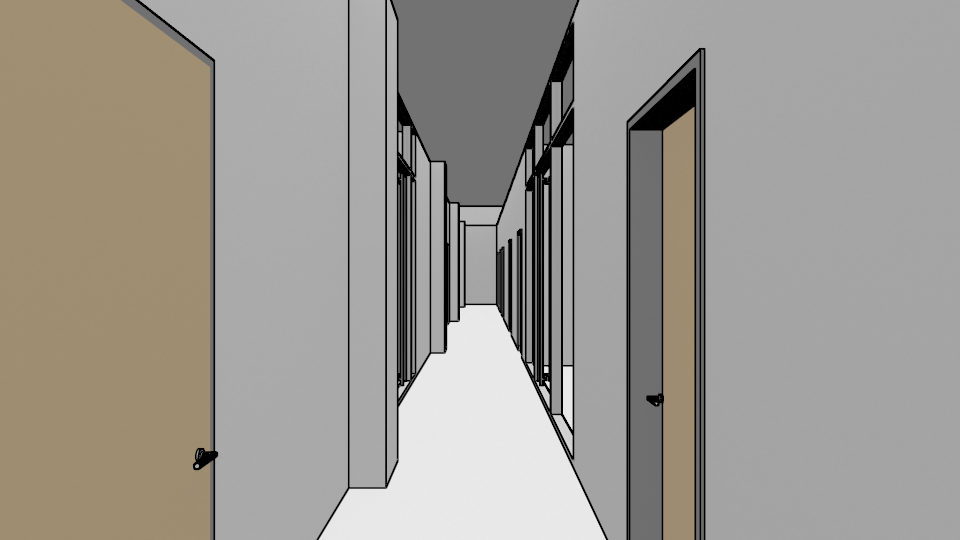
\includegraphics[width=\linewidth]{images/syn_dataset/e00708.png}
		\caption{synthetisches \hspace{1cm} Kantenbild}
		\label{subfig:edge}
	\end{subfigure}
	\hfill
	\begin{subfigure}[t]{0.24\linewidth}
		\centering
		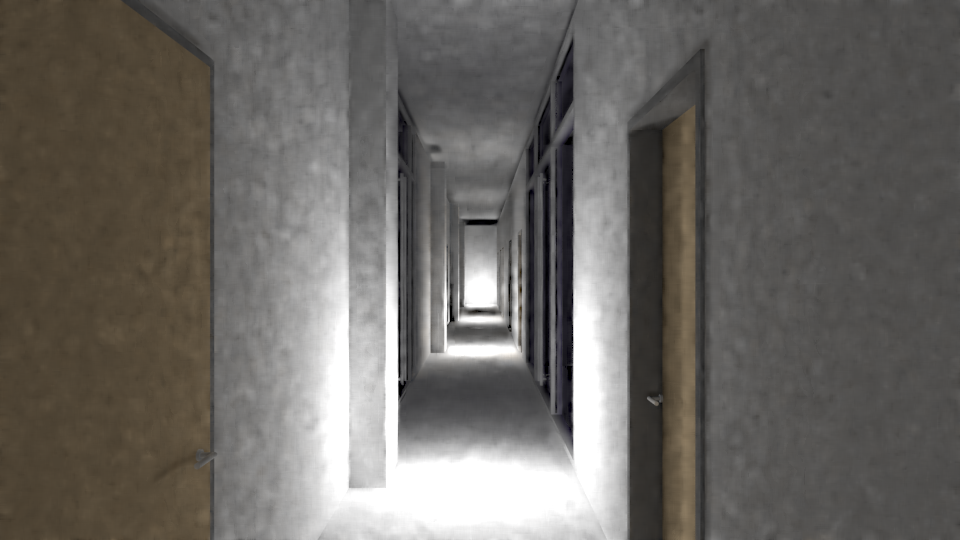
\includegraphics[width=\linewidth]{images/syn_dataset/c00708.png}
		\caption{fotorealistische \hspace{1cm} Simulation}
		\label{subfig:photorealistic}
	\end{subfigure}
	\hfill 
	\begin{subfigure}[t]{0.24\linewidth}
		\centering
		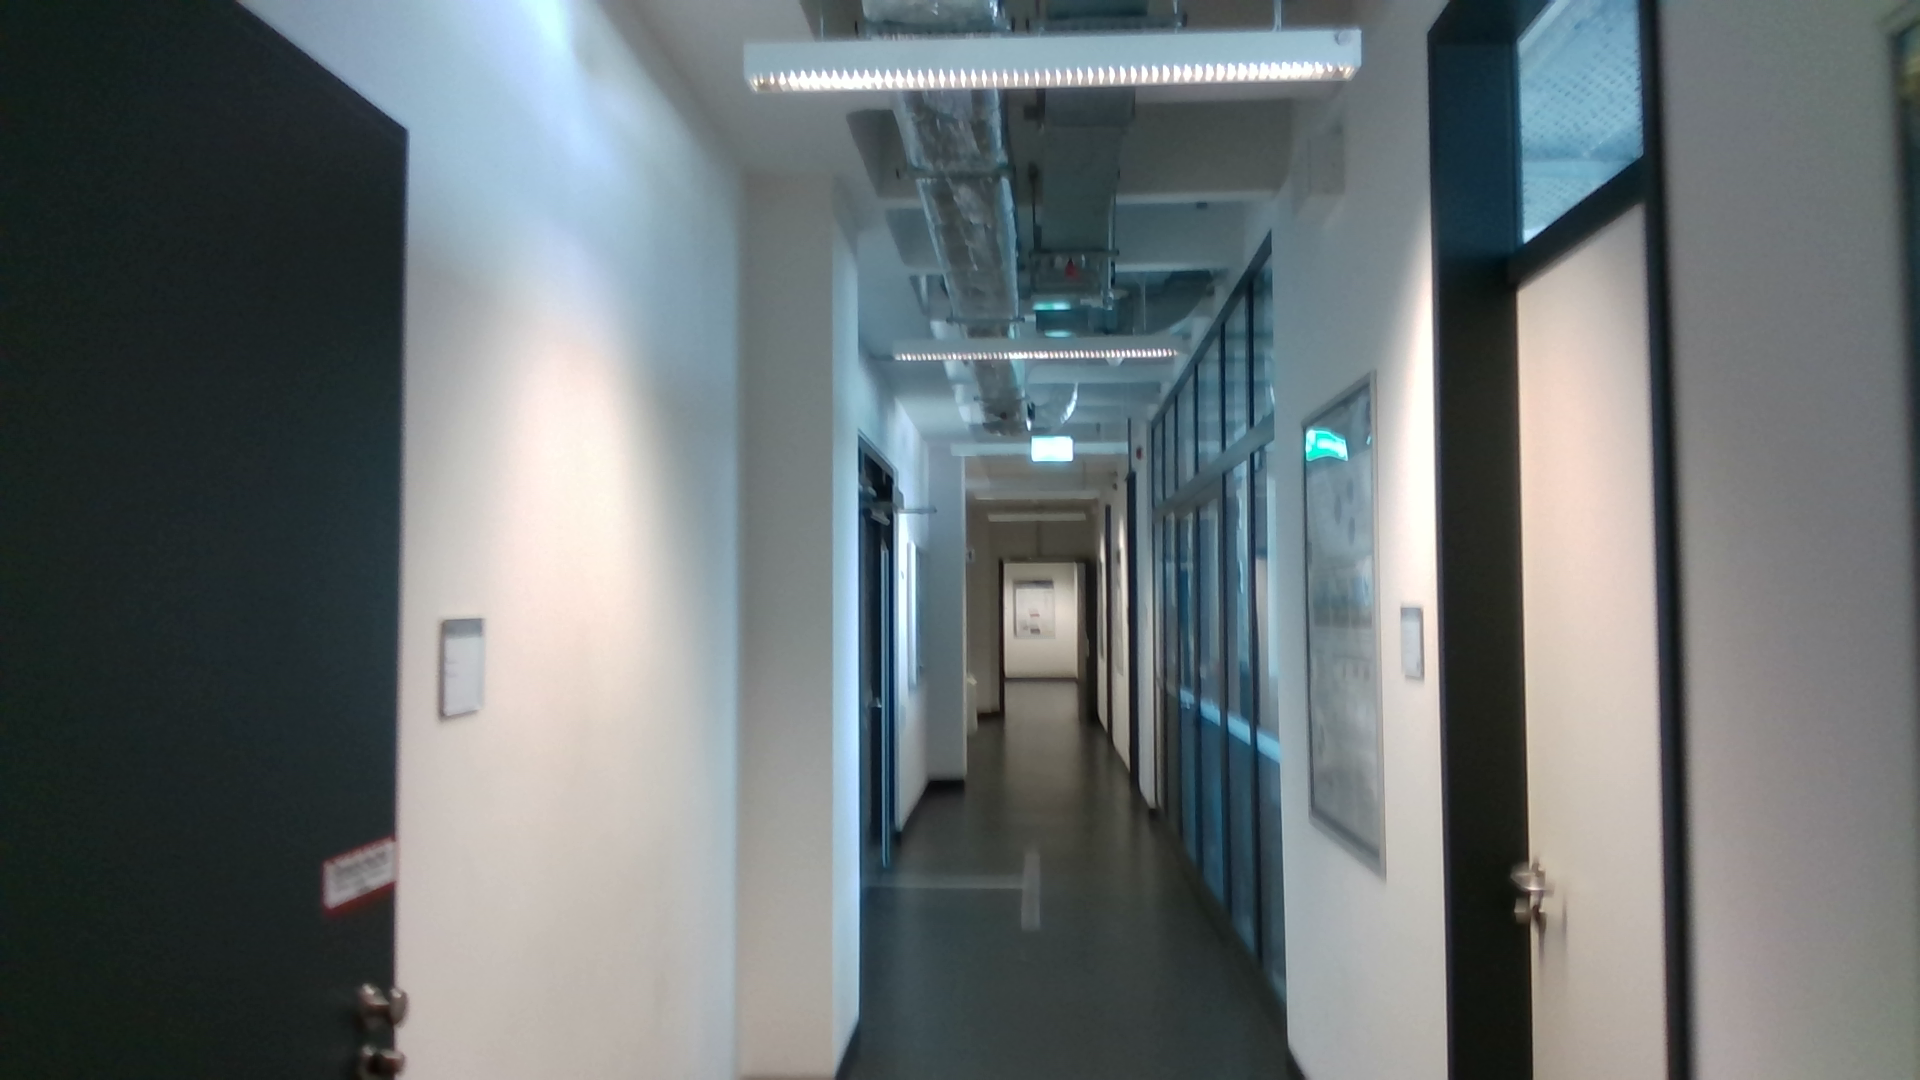
\includegraphics[width=\linewidth]{images/syn_dataset/r000305.png}
		\caption{reale Aufnahme}
		\label{subfig:real}
	\end{subfigure}
	\hfill 
	\begin{subfigure}[t]{0.24\linewidth}
		\centering
		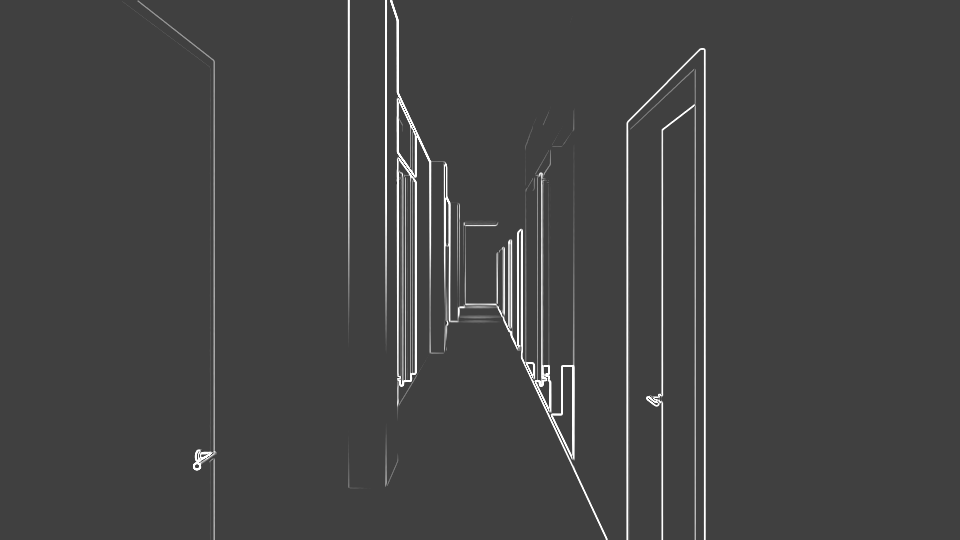
\includegraphics[width=\linewidth]{images/syn_dataset/bg00708.png}
		\caption{Gradientenbild  \hspace{1cm} von \ref{subfig:cartoonish}}
	\end{subfigure}
	\hfill
	\begin{subfigure}[t]{0.24\linewidth}
		\centering
		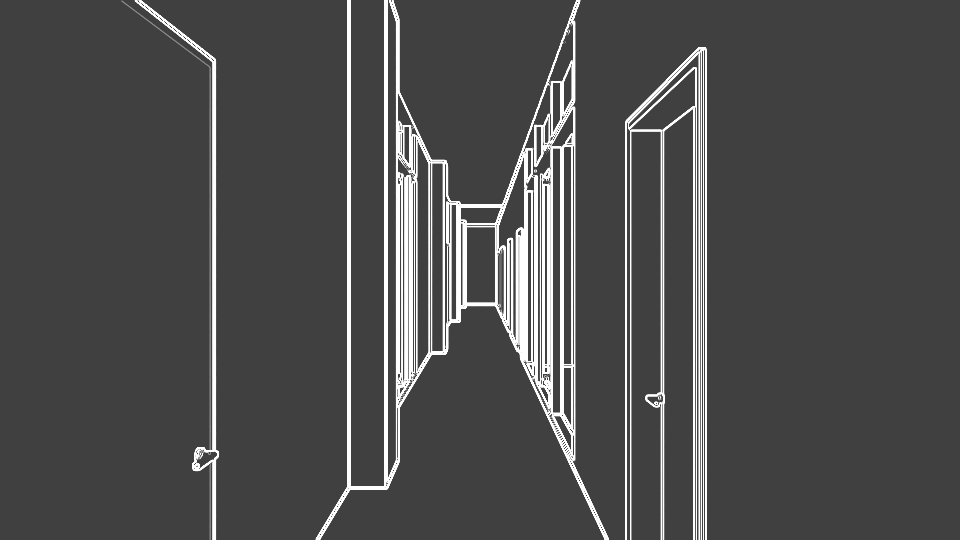
\includegraphics[width=\linewidth]{images/syn_dataset/eg00708.png}
		\caption{Gradientenbild  \hspace{1cm} von \ref{subfig:edge}}
	\end{subfigure}
	\hfill
	\begin{subfigure}[t]{0.24\linewidth}
		\centering
		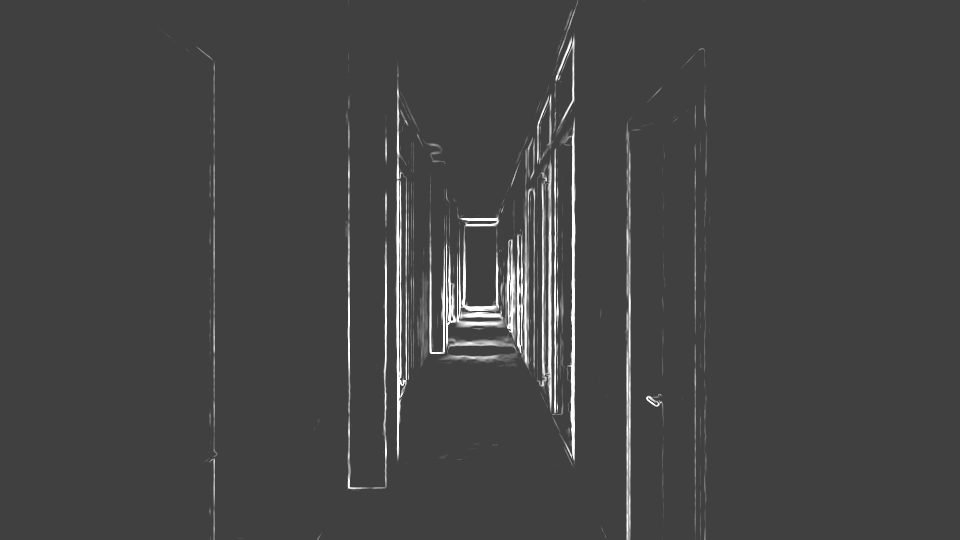
\includegraphics[width=\linewidth]{images/syn_dataset/cg00708.png}
		\caption{Gradientenbild  \hspace{1cm} von \ref{subfig:photorealistic}}
	\end{subfigure}
	\begin{subfigure}[t]{0.24\linewidth}
		\centering
		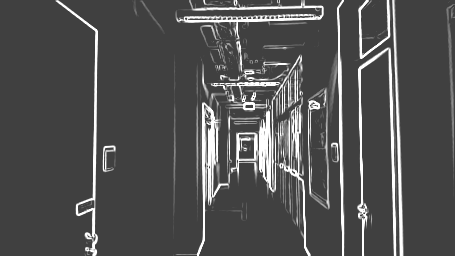
\includegraphics[width=\linewidth]{images/syn_dataset/rg000305.png}
		\caption{Gradientenbild  \hspace{1cm} von \ref{subfig:real}}
	\end{subfigure}
	\hfill
	\caption{Beispielhafte Bilder für jeden Datensatztyp und die dazu korrespondierenden Gradientenbilden.}
	\label{fig:dataset_preprocess}
\end{figure}
\vspace{\fill}

\subsection{Trainingsparameter}
Es wird die Caffe Implementierung \cite{jiaCaffeConvolutionalArchitecture2014} von PoseNet verwendet, die von den eigenen Autoren \citet{kendallPoseNetConvolutionalNetwork2015} veröffentlicht wurde.

Die Batchsize beträgt 40 und die Anzahl der Trainingsepochen ist 160. Eine NVIDIA GeForce GTX 1080 Ti mit 11GB Grafikspeicher wird verwendet und ermöglicht bei einer Batchsize von 40 drei Trainingsprozesse zeitgleich durchzuführen.

Der Hyperparameter $\beta$, der von PoseNet vorgestellten Kostenfunktion (vgl. Gleichung \ref{eq:posenet_loss}), wird durch ein Grid-Search Verfahren bestimmt, indem PoseNet mit der Hälfte der realen Daten trainiert und mit der restlichen Hälfte evaluiert wird. Der Wert von $\beta$ für den IC(TODO)-Datensatz beträgt 680 und das $\beta$ für das Seminargebäude ist $x$ (vgl. Abschnitt \ref{subsec:determine_beta}). Der Loss wird mit dem AdaGrad \cite{duchiAdaptiveSubgradientMethods2011} Gradientenabstiegsverfahren mit einer konstanten Lernrate von $10^{-3}$ optimiert bzw. minimiert. 

Die Trainings- sowie Testdaten werden auf eine Auflösung von $455\times256$ skaliert. Während des Trainingsprozesses werden zufällige Ausschnitte der Größe $224 \times 224$ aus dem skalierten Datensatz genommen und für die Evaluierung wird ein zentriertes Ausschnitt der selben Größe aus dem skalierten Testdatensatz verwendet. Das Durchschnittsbild der synthetischen Daten werden beim Trainieren und bei der Evaluierung von den Inputbildern subtrahiert.

Die Gewichte des Netzwerks werden mit den Gewichten eines Models initialisiert, das auf der GoogLeNet Architektur mit dem Places Datensatz \cite{zhouLearningDeepFeatures2014} trainiert wurde. Anschließend wird mit den synthetischen Daten trainiert und mit den realen Daten evaluiert. Die Tabelle \ref{tab:trainingparams} gibt eine Übersicht der Hyperparameter an.

\begin{table}[H]
	\centering
	\caption{Übersicht der Hyperparameter.}
	\begin{tabularx}{1.0\textwidth}{X X}
		\textbf{Hyperparameter} & \textbf{Wert}\\
		\hline
		Batchsize & $40$\\
		\hline
		Anzahl der Epochen & $160$\\
		\hline
		$\beta$ der Kostenfunktion (vgl. Gleichung \ref{eq:posenet_loss}) &
		\makecell[tl]{
			$680$ für 1 TODO\\
			$x$ für 2 (vgl. Abschnitt \ref{subsec:determine_beta})\\
		}\\
		\hline
		Loss-Optimierer & AdaGrad\\
		\hline
		Lernrate & $10^{-3}$\\
		\hline
		Bildskalierung & $455 \times 256$\\
		\hline
		Bildausschnitt& \makecell[tl]{
			$224 \times 244$\\
			(Training: zufällig, Evalution: zentriert)\\
		}\\
		\hline
		Datensatznormierung & Subtraktion des Durchschnittsbildes der synthetischen Daten \\
		\hline
		Initialisierung der Gewichte & Gewichte eines mit dem Places Datensatz trainierten Models auf GoogLeNet \\
	\end{tabularx}
	\label{tab:trainingparams}
\end{table}